\documentclass[11pt]{article}

\usepackage{latexsym}
\usepackage{graphicx}
\usepackage{amssymb}
\usepackage{amsthm}
\usepackage{enumerate}
\usepackage{amsmath}
\usepackage{cancel}

\setlength{\evensidemargin}{.25in}
\setlength{\oddsidemargin}{-.25in}
\setlength{\topmargin}{-.75in}
\setlength{\textwidth}{6.5in}
\setlength{\textheight}{9.5in}
\newcommand{\due}{September 12th, 2015}
\newcommand{\HWnum}{1}
\input{"C:/Users/joeor_000/Documents/Coursework/Define.tex"}

\begin{document}
\begin{figure}
\centering
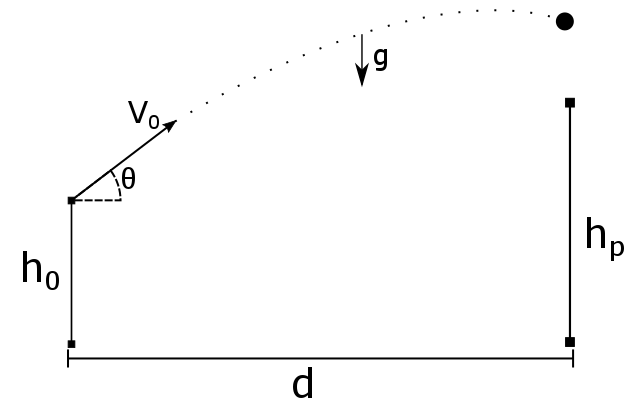
\includegraphics[width=0.8\textwidth]{Figure.png}
\caption{}
\label{figure}
\end{figure}

To solve this problem we first draw a sketch so we can identify the relevant details of the 
problem. This sketch is shown in figure \ref{figure}.


\section{Motion of the Ball}
Now, in order to solve for the time of the jump $t_{jump}$ we need to first determine the 
motion of the ball. In order to do this we start from the fact that we know the ball is
under a constant acceleration, $g$, in the downwards direction. Note we will define 
downwards as the negative direction, so we integrate to find $v^{ball}_{y}(t)$ by
\begin{align*}
a^{ball}_y(t) &= \frac{dv^{ball}_{y}(t)}{dt} = -g\\
&\Downarrow\\
\int dv^{ball}_{y}(t) &= \int-gdt\\
v^{ball}_y(t) &= -gt + A
\end{align*}
We determine $A$ by the initial condition of the velocity in the $y$ direction. Before we solve for $A$ we need to 
determine what the velocity of the ball is at $t=0$. The problem states that the ball is 
thrown at a velocity, $v_0$, at an angle $\theta$. Therefore we need to find the 
$y$-component of $v_0$ which is given by 
$$v^{ball}_{0y} = v_0\sin\theta$$
So, we can determine $A$ by
\begin{align*}
v^{ball}_y(t=0) = v_0\sin\theta &= -g(0) + A\\
&\Downarrow\\
A &= v_0\sin\theta
\end{align*}
This gives us the equation for the velocity of the ball in the $y$-direction
\begin{equation}
v^{ball}_{y}(t) = v_0\sin\theta - gt.
\label{VYBall}
\end{equation}
Using equation \ref{VYBall} we can then find the functional form of the $y$ position by
the integral
\begin{align*}
v^{ball}_y &= \frac{dy^{ball}(t)}{dt}\\
&\Downarrow\\
\int dy^{ball}(t) &= \int v^{ball}_{y}(t)dt\\
&= \int v_0\sin\theta - gt dt\\
&= v_0\sin\theta t - \frac{1}{2}gt^2 + B
\end{align*}
Again we need to determine the constant of integration by applying the fact that the ball is 
initially thrown at a height, $h_0$. This gives the initial condition $y^{ball}(t=0) = h_0$.
Which allows us to solve for $B$ by
\begin{align*}
y^{ball}(t=0) = h_0 &= v_0\sin\theta(0) - \frac{1}{2}g(0)^2 + B\\
&\Downarrow\\
B &= h_0
\end{align*}
Which gives us the equation for the $y$-component of the ball
\begin{equation}
y^{ball}(t) = h_0 + v_0\sin\theta t - \frac{1}{2}gt^2
\end{equation}
Next we need to find the dynamical equations in the $x$ direction. We assume that there is 
no air resistance which implies that $a^{ball}_{x} = 0$. Therefore we can find the equation 
for the velocity in the $x$-direction by integrating
\begin{align*}
a^{ball}_x(t) &= \frac{dv^{ball}_x}{dt}\\
&\Downarrow\\
\int dv^{ball}(t)_x &= \int a^{ball}_x(t)dt\\
v^{ball}_x(t) &= \int 0 dt\\
v^{ball}_x(t) &= C
\end{align*}
Note that because we have no acceleration we found that the velocity is constant in time.
So we need to determine $C$ again by initial conditions. Like before we realize that when a
ball is throw with velocity $v_0$ at an angle $\theta$ it has a component in the $x$ 
direction given by
$$v^{ball}_x(t=0) = v_0\cos\theta.$$
Now it is easy to see that $C=v_0\cos\theta$ because as we have said before the velocity is 
constant for all time. This implies that the initial velocity is the velocity in the $x$
direction for all time. So we have
\begin{equation}
v^{ball}_x(t) = v_0\cos\theta
\label{VXBall}
\end{equation}
which we can use to find the function for the $x$ position. Like before we have
\begin{align*}
v^{ball}_x(t) &= \frac{dx^{ball}(t)}{dt}\\
&\Downarrow\\
\int dx^{ball}(t) &= \int v^{ball}_x(t)dt\\
x^{ball}(t) &= \int v_0\cos\theta dt\\
x^{ball}(t) &= v_0\cos\theta t + D
\end{align*}
To find $D$ we assume that we throw the ball from an initial position $x_0$ which implies 
that $x^{ball}(t=0) = x_0$. Which solving for $D$ yields
\begin{align*}
x^{ball}(t=0) = x_0 &= v_0\cos\theta (0) + D\\
&\Downarrow\\
D&=x_0
\end{align*}
Which gives the equation for the $x$ position of the ball as
\begin{equation}
x^{ball}(t) = x_0 + v_0\cos\theta t
\label{XBall}
\end{equation}
So we can collect the equations that define the motion of the ball
\begin{align*}
v^{ball}_{y}(t) &= v_0\sin\theta - gt\\
y^{ball}(t) &= h_0 + v_0\sin\theta t - \frac{1}{2}gt^2\\
v^{ball}_x(t) &= v_0\cos\theta\\
x^{ball}(t) &= x_0 + v_0\cos\theta t
\end{align*}
Now we can look at the details of the problem as see that we want to determine the height of
the ball, $y^{ball}(t)$, when it has traveled a distance $d$ away from the thrower in the $x$
direction. To do this we look at $x^{ball}(t)$ to determine how long it takes the ball to 
travel a distance $d$ from the thrower. We can write this mathematically as 
$x^{ball}(t=t_d) = x_0+d$. So we can solve for the balls travel time, $t_d$, by 
\begin{align*}
x^{ball}(t=t_d) = x_0+d &= x_0 +v_0\cos\theta t_d\\ 
x_0+d-x_0 &= x_0 +v_0\cos\theta t_d -x_0\\ 
d &= v_0\cos\theta t_d \\ 
&\Downarrow\\
t_d &= \frac{d}{v_0\cos\theta}
\end{align*}
Now that we know the ball's travel time we can find how high the ball is at this time by
\begin{align*}
y^{ball}(t=t_d) &= h_0 + v_0\sin\theta t_d - \frac{1}{2}gt_d^2\\
&= h_0 + v_0\sin\theta \frac{d}{v_0\cos\theta} - \frac{1}{2}g\left(\frac{d}{v_0\cos\theta}\right)^2\\
&= h_0 + d\tan\theta - \frac{1}{2}g\left(\frac{d}{v_0\cos\theta}\right)^2
\end{align*}
By solving for this we know know how high the catcher is going to need to jump. We can use 
this result in the next section.

\section{Motion of the Catcher}
To find how long the catcher is in the air for we first need to derive the equations for 
the catcher's motion. We assume that the catcher jumps exactly vertically this means we only 
have to consider the $y$ component of their motion. Because the ball and the catcher are on 
the same planet we can say that they both feel the same acceleration $a^{catch}(t) = -g$.
Using this we can derive equations of motion by integrating
\begin{align*}
a^{catch}(t) &= \frac{dv^{catch}(t)}{dt}\\
&\Downarrow\\
\int dv^{catch}(t) &= \int a^{catch}(t)dt\\
v^{catch}(t) &= \int -gdt\\
v^{catch}(t) &= -gt + E
\end{align*}
Were we find $E$ by the initial condition $v^{catch}(t=0) = v^{catch}_0$. Note because we split the
problem into two different parts we define a new reference for time. So we can solve for $E$
\begin{align*}
v^{catch}(t=0) = v^{catch}_0 &= -g0 + E\\
&\Downarrow\\
E &= v^{catch}_0
\end{align*}
So our catchers velocity is given by
\begin{equation}
v^{catch}(t) = v^{catch}_0 - gt
\label{VCatch}
\end{equation}
And like before we can integrate $v^{catch}(t)$ to find the equation for the height of the 
catcher.
\begin{align*}
v^{catch}(t) &= \frac{dy^{catch}(t)}{dt}\\
&\Downarrow\\
\int dy^{catch}(t) &= \int v^{catch}(t)dt\\
y^{catch}(t) &= \int v^{catch}_0-gtdt\\
y^{catch}(t) &= v^{catch}_0t-\frac{1}{2}gt^2+F
\end{align*}
And we find $F$ by apply the initial condition that $y^{catch}(t=0) = h_p$ which gives
\begin{align*}
y^{catch}(t=0) = h_p &= v^{catch}_0(0)-g(0)^2+F\\
&\Downarrow\\
F &= h_p
\end{align*}
which yields the equation of motion 
\begin{equation}
y^{catch}(t) = h_p + v^{catch}_0t - \frac{1}{2}gt^2.
\label{YCatch}
\end{equation}
Now we need to consider what is happening at $t_{jump}$. We want the catchers height to be 
the height of the ball we found in the previous part. Which we can write mathematically as 
the condition
$$y^{catch}(t=t_{jump}) = h_0 + d\tan\theta - \frac{1}{2}g\left(\frac{d}{v_0\cos\theta}\right)^2  = h_p + v^{catch}_0t_{jump} - \frac{1}{2}gt_{jump}^2$$
We are really close to finding $t_{jump}$, the final missing piece we need is to find 
velocity the catcher uses to leave the ground, $v^{catch}_0$. To find this we realize that 
we want the catcher to be at the top of their jump right when they catch the ball. This 
implies that the catcher's velocity at the end of his jump is zero. Which we write as the 
constraint $v^{catch}(t=t_{jump}) = 0$ which allows us to solve
\begin{align*}
v^{catch}(t=t_{jump}) = 0 &= v^{catch}_0 - gt_{jump}\\
&\Downarrow\\
v^{catch}_0 &= gt_{jump}\\
\end{align*}
Note that $t_{jump}$ is a specific constant time not to be confused with the general $t$. 
This distinction keeps $v^{catch}_0$ a constant. So now we can solve for $t_{jump}$ by 
using $y^{catch}(t)$
\begin{align*}
y^{catch}(t=t_{jump}) = h_0 + d\tan\theta - \frac{1}{2}g\left(\frac{d}{v_0\cos\theta}\right)^2  &= h_p + v^{catch}_0t_{jump} - \frac{1}{2}gt_{jump}^2\\
&\Downarrow\\
h_0 + d\tan\theta - \frac{1}{2}g\left(\frac{d}{v_0\cos\theta}\right)^2  &= h_p + (gt_jump)t_{jump} - \frac{1}{2}gt_{jump}^2\\
h_0 + d\tan\theta - \frac{1}{2}g\left(\frac{d}{v_0\cos\theta}\right)^2  &= h_p + gt_{jump}^2 - \frac{1}{2}gt_{jump}^2\\
h_0 - h_p + d\tan\theta - \frac{1}{2}g\left(\frac{d}{v_0\cos\theta}\right)^2  &= h_p - h_p + \frac{1}{2}gt_{jump}^2\\
2\left(h_0 - h_p + d\tan\theta - \frac{1}{2}g\left(\frac{d}{v_0\cos\theta}\right)^2\right)  &= 2\frac{1}{2}gt_{jump}^2\\
\frac{1}{g}2\left(h_0 - h_p + d\tan\theta - \frac{1}{2}g\left(\frac{d}{v_0\cos\theta}\right)^2\right)  &= \frac{1}{g}gt_{jump}^2\\
&\Downarrow\\
\frac{2\left(h_0 - h_p + d\tan\theta - \frac{1}{2}g\left(\frac{d}{v_0\cos\theta}\right)^2\right)}{g}  &= t_{jump}^2\\
&\Downarrow\\
t_{jump} &= \sqrt{\frac{2\left(h_0 - h_p + d\tan\theta - \frac{1}{2}g\left(\frac{d}{v_0\cos\theta}\right)^2\right)}{g}}
\end{align*}
As an extra exercise try the solving this problem using this method but with the added 
complication with a time dependent gravity when $-g\rightarrow -Ct$ where $C$ is a positive
constant. And see if you can find the expression for $t_{jump}$ as
$$t_{jump} = \sqrt[3]{\frac{3\left(h_0 - h_p + d\tan\theta - \frac{1}{2}g\left(\frac{d}{v_0\cos\theta}\right)^2\right)}{C}}$$


\end{document}
